\chapter{Introducción}
\label{ch:intro}

En este capítulo, se introduce al lector en el dominio de las apuestas deportivas en Internet y se presenta el terminal elegido como plataforma de la aplicación de apuestas, resultado del presente trabajo de fin de carrera.

\section{Apuestas por Internet}

%\fxnote{``Mundo de la apuestas'' es demasiado genérico}

%\fxnote{Yo hablaría de apuestas, de casas de apuestas tradicionales y de su entrada en Internet. Pondría ejemplos sobre lo que se puede y no se puede hacer para que el lector se familiarice.}

%\fxnote{Luego hablaría del concepto de ``casa de intercambios'' en las que el ``bookie'' no es la casa si no cualquier otro apostador. La idea, como dices en algún momento es simple: los apostadores pueden apostar a favor (significado habitual de apostar) o en contra (con el significado de cubrir una apuesta a favor).}

%\fxnote{Recuerda este enlace en el que hay dos documentos que creo que pueden ayudar con esta presentación del dominio del problema: \url{http://www.iapuestas.com/Guia/introduccionintercambiodeapuestas.asp} y \url{http://www.iapuestas.com/Guia/lasmatematicasdelasapuestas.doc}. Quizá pueda salir algo de \url{http://www.sportsbookreview.com/Espanol/Default.aspx}, \url{http://internetgamblingreport.com/ o http://anjaander.blogspot.com/} o incluso \url{http://en.wikipedia.org/wiki/Bet_exchange}}

Actualmente las apuestas tienen gran aceptación en todo el mundo. En España ya hay una tradición de bastantes años por la quiniela y la lotería. En la quiniela, por ejemplo, nunca sabemos por anticipado cuánto cobraremos en caso de acierto ya que depende del número de participantes que hayan acertado el resultado de la jornada de la Liga Profesional de Fútbol. Un acierto de 13 resultados puede convertirse en una gran decepción por el premio conseguido si junto con nosotros han acertado el resultado otras 100 personas. Sin embargo, si eres el único acertante ya no tienes que repartir el premio. En las casas de apuestas tradicionales el apostante cruza su apuesta directamente contra la propia casa. En un típico ejemplo tenemos las clásicas carreras de caballos sobre las que se apuesta sobre un caballo ganador. La casa de apuesta tradicional se limita siempre a cubrir nuestras apuestas. 


En los últimos años hemos sido testigos de la llegada de las llamadas casas de intercambio. 
%\fxnote{no creo que estén desfasadas} 
% \fxnote{Tb. puedes decir que la casa ``cubre'' la apuesta.}. 
Las casas de intercambio añaden un nuevo concepto en el mundo de las apuestas. Los usuarios realizan las apuestas sobre los eventos y entre ellos mismos se cubren las apuestas, es decir, los apostantes pueden realizar apuestas a favor o en contra de los eventos. 
%\fxnote{Falso, las cuotas y cantidades a apostar existen siempre}
 En este caso, la casa de apuestas hace de intermediario obteniendo un porcentaje en la ganancia del apostante. %\fxnote{Creo que hace falta decir que los apostantes apuestan a favor y en contra} 
 Las ventajas de las casas de apuestas de intercambio con respecto a las tradicionales son:
\begin{itemize}
	\item Las comisiones son menores que las correspondientes a una casa de apuestas tradicionales.
	\item Cuanto mayores sean las cantidades apostadas, mayor será la comisión que se lleve la casa de intercambio, es por eso que no suelen existir límites en las cantidades a apostar en contra de las casas de apuestas tradicionales siempre y cuando se cubra una apuesta a favor con otro en contra.%\fxnote{Pero existen límites que pueden ser inferiores a los de las casas normales, si nadie apuesta en contra o a favor, por ejemplo.}
\end{itemize}
Pero como en toda comparación siempre hay desventajas: 
\begin{itemize}
	\item Normalmente, debido a las nuevas posibilidades de apuesta de las casas de intercambio se requieren conocimientos avanzados y una mayor experiencia para obtener beneficios en contraposición a la simplicidad que ofrecen las casas de apuestas tradicionales.
	\item En las casas de intercambio son los propios usuarios los que proponen sus apuestas y los mercados tardan más tiempo en abrirse. Entendemos por mercado el evento deportivo por el cual podemos apostar a favor o en contra. Por ejemplo, en un partido de tenis apostar por cúal de los dos jugadores va a ganar. En las casas de apuestas tradicionales es la propia casa la que establece las cuotas abriendo los mercados más rápidamente.
\end{itemize}

Debido a la aparición de estas casas de intercambio, aparecen dos nuevas modalidades para realizar apuestas. La primera el poder realizar apuestas en contra de un evento (\emph{lay})  diferenciándose claramente de las casas de apuestas tradicionales donde sólo se pueden realizar apuestas a favor (\emph{back}) de un evento.
 La segunda modalidad es la facilidad para realizar \emph{trading}, concepto que desarrollaremos en el siguiente apartado.
 %\fxnote{El trading es algo que tb se puede hacer en las casas normales, habitualmente utilizando varias casas}  

 \subsection{Apuestas Back y Lay}
 
   Para un mejor entendimiento y comprensión de la temática de este trabajo de fin de carrera, definiremos los principales conceptos en una apuesta:
 \begin{itemize}
 \item Bankroll: es la cantidad de dinero o capital  que estamos dispuestos a apostar. Lógicamente tendremos que administrarlo de la mejor manera posible, minimizando las pérdidas en caso de perder una apuesta y maximizar las ganancias de una apuesta ganadora. La disciplina y el conocimiento del mercado son las mejores aliadas de nuestro bankroll. La mayoría de las casas de apuestas por Internet nos regalan un mínimo bankroll para animarnos a participar en ellas.
 \item Stake: es la cantidad de dinero que ofrecemos por un determinado evento en la apuesta . Es decir, apostar 10 euros a que gana el Sevilla F.C el campeonato de la Liga Profesional de Fútbol.
 \item Odds: es la cuota (probabilidad) de una apuesta. Por ejemplo se paga una cuota de 3 a 1 que Fernando Alonso gane el mundial de Fórmula 1. Nos refleja que Fernando Alonso tiene más probabilidades de ganar el campeonato que no ganarlo.
 \item Beneficio: es la ganancia que obtenemos de una apuesta ganadora cuyo cálculo es el siguiente:
 \begin{displaymath}
 Beneficio = (stake \times odd) - stake 
\end{displaymath}

%\begin{anfxnote}
%  Latex es famoso por la potencia a la hora de escribir fórmulas   matemáticas:
%
%\begin{displaymath}
%  B = s \times o
%\end{displaymath}
%
%\end{anfxnote}

\item Pérdida: lógicamente lo opuesto al beneficio. Lo que todo apostante quiere evitar o minimizar. 
\item Yield: expresado en porcentaje. Nos indica el beneficio obtenido del total apostado. Es lo que diferencia a un buen apostador del resto. El cálculo es el siguiente:
\begin{displaymath}
 Yield = (beneficio / total apostado) \times 100 
\end{displaymath}
\end{itemize} 


 
 \subsection{Trading}
 
 Se trata de apostar a favor y en contra sobre un mismo evento obteniendo así una ganancia segura en unos casos o minimizar la pérdida en otros.  Esta modalidad se puede realizar en la casa de apuestas tradicionales pero para ello necesitas usar varias casas. Es decir, en una casa cubre la apuesta a favor de un evento mientras que otra casa ve más interesante cubrir la opuesta. Este término también se suele usar en operaciones financieras, como por ejemplo la Bolsa.
  
  
  Este método se suele dar en dos escenarios típicos:
  
  
\begin{itemize}
	\item Ganancia segura.
	  Se suele llamar apuesta segura, es decir cualquiera que sea el desenlace del evento, nunca se pueda perder. La condición necesaria para ello es que la cuota de la apuesta a favor sea superior a la cuota de la apuesta en contra. 
	\item Minimizar la pérdida.
	   Lo contrario que el punto anterior. Es decir, el mercado evoluciona de tal manera que la cuota de la apuesta en contra es mayor que la ya realizada a favor. En este caso lo que se persigue es minimizar la pérdida segura.
\end{itemize}


A continuación exponemos un ejemplo de caso típico de \emph{trading}.
%\begin{figure} [h]
%  \centering
%    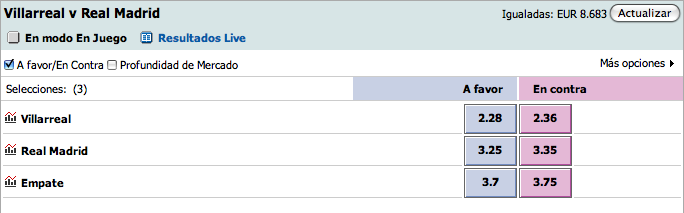
\includegraphics[width=0.6\textwidth]{./images/SampleTrading1.png}
%  \caption{Situacion inicial}
%  \label{fig:Inicio}
%\end{figure}
 Nos basaremos en las apuestas deportivas sobre un partido de tenis.
 
 \begin{center}
    \begin{tabular}{| c | c | c |}
      \hline
      \hline
      players & A favor & En contra\\
      \hline
      \hline
      Rafa Nadal & 2.18 & 2.2\\
      \hline
      \hline
      Roger Federer & 1.8 & 1.85\\
      \hline
      \hline
    \end{tabular}
  \end{center}

%\fxnote{Hay que explicar el significado de la figura, ¿qué son esos números? ¿qué significan?}

En la tabla
% \fxnote{En Latex jamás escribes un número, todo son referencias: \ref{fig:Inicio}}, 
podemos ver las cuotas a favor y en contra de un partido de tenis entre Rafa Nadal y Roger Federer. La cuota a favor de Rafa Nadal está mucho más alta que la de Roger Federer.  En el mundo de las apuestas, influyen todos los pequeños factores que al aficionado se les escapa. Supongamos que Nadal gana los dos primeros sets, esto desemboca en cambios en la tabla de apuestas. 

  Vemos ahora que el mercado ha cambiado. Ahora la cuota de Nadal a bajado claramente.
   
 \begin{center}
    \begin{tabular}{| c | c | c |}
      \hline
      \hline
      players & A favor & En contra\\
      \hline
      \hline
      Rafa Nadal & 1.2 & 1.5\\
      \hline
      \hline
      Roger Federer & 1.8 & 1.3\\
      \hline
      \hline
    \end{tabular}
  \end{center}
  
  
  %\begin{figure} [h]
   % \centering
   %    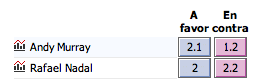
\includegraphics[width=0.6\textwidth]{./images/SampleTrading2.png}
   %  \caption{Situacion cambiante}
   %\label{fig:Inicio}
%\end{figure}
En las apuestas, al estar ligas claramente a estadísticas, nunca podemos asegurar un resultado por muchas condiciones favorables que se den. En este caso, debido a que es un partido con dos jugadores de primer nivel, tenemos la ocasión de asegurar beneficios si apostamos en contra de Nadal. Aunque pueda parecer raro, siempre puede haber condiciones que afecten claramente a los resultados como por ejemplo una lesión de Nadal.

Al inicio del ejemplo realizamos una apuesta a favor de Rafa Nadal por 50 euros, con lo que tendríamos:

%\fxnote{¿Por qué apostar a favor de Nada? ¿Sabemos algo que nadie sabe? ¿Intuímos algo? ¿Tenemos datos estadísticos?}   	
	 
\begin{displaymath}
  Beneficio = (2.18 \times 50) - 50 =  59 \euro  
\end{displaymath}

Por lo que tenemos 59 euros si ganal Nadal, en caso contrario:
 
 \begin{displaymath}
  Riesgo = - 50 \euro 
\end{displaymath}
Tendremos una pérdida de 50 euros si pierda Nadal.
	
Un tiempo más adelante, el mercado ha cambiado debido al resultado de los dos primeros set, Nadal ya es favorito pero queremos asegurarnos un beneficio seguro.
  
Para asegurar el dinero apostado anteriormente realizamos una apuesta en contra de Nadal. De tal forma que nos queda:
  \begin{displaymath}
  Beneficio = 60 \euro 
  \end{displaymath} euros si pierde Nadal.
   \begin{displaymath}
  Riesgo = 60 - (1.5 \times 60) = -30 \euro
  \end{displaymath} euros si gana Nadal.
  
	 
Al final si gana Rafa Nadal obtenemos: 
   \begin{displaymath}
   59 - 30 = 29 \euro 
   \end{displaymath}
   
Si pierde Nadal y por tanto gana Roger Federar tenemos:
   
  \begin{displaymath}
  60 - 50 = 10 \euro
  \end{displaymath}
       
   Con lo que estamos cubiertos ante cualquier resultado del partido. En ambos casos tenemos ganancias. 
   
   El escenario expuesto es uno de los mejores casos que nos pueden dar ya que obtenemos beneficio en ambos casos. Pero puede suceder que hayamos apostado por un evento con demasiada confianza y luego en un futuro vemos que puede ser una ruina. En ese escenario, el objetivo prioritario sería minimizar la pérdida apostando en contra del evento en cuestión.

 Las casas de apuestas nos ofrecen una gran variedad de apuestas en diferentes deportes que nos permiten adecuarnos a nuestros gustos y conocimientos. 

   
\section{Betfair}

 Debido al gran desarrollo de Internet en los principios de siglo empiezan a aparecer las primeras casas de intercambio %\fxnote{Casas de apuestas y casa de intercambio, creo que son dos concpetos diferentes, bwin es una casa de apuestas tradicional, betfair es una casa de intercambios de apuestas}
  online. Betfair\footnote{\url{www.betfair.com}}, Bwin\footnote{\url{www.bwin.com}}, Miapuesta.com\footnote{\url{http://www.miapuesta.com}} son ejemplos de casas afianzadas en Internet. % \fxnote{Ésto que dices no está claro: \url{http://www.sportsbookreview.com/Espanol/Default.aspx}}.
   Dentro de este grupo selecto aparece Betfair.%\fxnote{No creo que sea cierto y si lo es necesitamos una fuente fiable. Tenemos que tener cuidado, hemos de contrastar la información. ¿En qué sentido es la más grande?}.
 
%\fxnote{Please, menos marketing. Esto es un TFC, un documento eminentemente técnico.}

 Betfair fue fundado en Junio del año 2000. Es una de las primeras casas de apuestas online en ofrecer la modalidad de apuestas a favor y en contra de un evento. En el año 2007 la casa ya cuenta con más de 1.000.000 de usuarios generando un volumen de negocio de más de 50 millones de libras a la semana. Rápidamente se expande en más de 120 países de todo el mundo ofreciendo un portal web en 18 idiomas que gestiona más de 5 millones de transacciones al día. %\fxnote{Fuente?}

%\fxnote{No deberíamos explicar antes que el interfaz es Web y que e 2007 bla bla bla?}

En el año 2007, Betfair es el primer portal de apuestas que ofrece un API\footnote{Application Programming Interface} %\fxnote{Footnote demasiado largo}
 de acceso a sus servicios. El API de Betfair lo explicaremos con más detalle en el capítulo \ref{ch:diseno}. La estrategia es clara, enganchar a los desarrolladores para crear todo tipo de aplicaciones usando su portal de apuestas como base y que se adapten a cualquier dispositivo sea tanto un ordenador personal, agenda electrónica o dispositivo móvil. Como era de esperar, empezaron a salir multitud de aplicaciones, sobre todo dirigidas al sector de usuarios expertos en apuestas. Ahora, con las nuevas tecnologías móviles, el usuario busca realizar consultas en todo momento de sus servicios contratados. Ya sea email, servicios del banco, entradas de cine\ldots %\fxnote{\ldots para poner puntos susepnsivos} 
% \fxnote{Esta última frase quedaría mejor para lo del iPhone}

%\fxnote{Has pasado muy de puntillas por lo del API de BF y parece importante para tu TFC.}

\section{Apple y su terminal móvil iPhone}
 
Apple Computer, Inc. es una empresa estadounidense de tecnología informática fundada en 1976. Inició sus trabajos sobre los ordenadores personales en la década de los setenta con el ordenador Apple II y reinventó el ordenador personal en los ochenta con el Macintosh. Hoy en día, Apple es considerada como una de las principales empresas líderes en innovación con sus ordenadores.  %\fxnote{Please, menos marketing.}

El 23 de octubre de 2001, Apple decidió introducirse en la industria musical con su famoso reproductor de música \emph{iPod} y su tienda de discos \emph{iTunes}.

El 9 enero del año 2007 presenta su primer terminal móvil llamado \emph{iPhone}. Tal y como lo hizo años atrás en la industria musical, su terminal se hizo famoso en la industría de la telefonía móvil por su diseño, su sistema operativo \emph{iPhone OS} y la introducción de nuevas tecnologías como la pantalla táctil.

\begin{figure} [h]
  \centering
    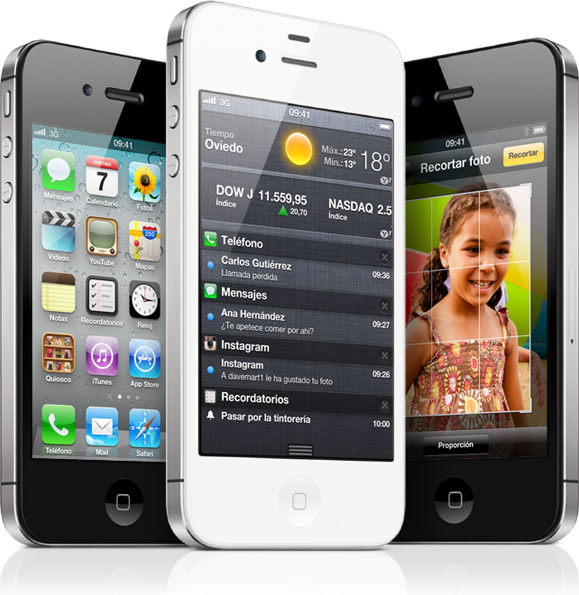
\includegraphics[width=0.6\textwidth]{./images/iphone4.jpg} 
  \caption{iPhone 4GS}
  \label{fig:iPhone-4GS}
\end{figure}
  
  En marzo de 2008 Apple muestra una nueva versión del terminal con tecnología 3G y comunica el lanzamiento de su propia tienda de aplicaciones para el iPhone, la \emph{iTunes application store}. Para nutrir esa tienda de aplicaciones  lanza un conjunto de herramientas de desarrollo iPhone SDK\footnote{Software Development Kit} para todos aquellos desarrolladores que quieran participar en la misma. En el capítulo \ref{ch:diseno}  explicamos con más detalle dicho SDK ya que es una pieza clave en el presente trabajo de fin de carrera. %\fxnote{Y sin embargo esta parte es fundamental: ¿Qué es el SDK? ¿Cómo es? ¿Quién puede usarlo? ¿Cómo se programa? etc. etc. etc.}
  
   Otro hito importante a destacar ocurre el 27 de enero de 2010. Apple amplía la familia de dispositivos con una tableta táctil de 10 pulgadas denominada \emph{iPad}. Misma filosofía pero ahora en formato de pantalla más grande. De la misma forma que evoluciona sus dispositivos, evoluciona el \emph{SDK} para ofrecer a los desarrolladores las herramientas necesarias para crear aplicaciones compatibles entre la familia de dispositivos. A partir de 2010 el sistema operativo de los dispositivos para a denominarse \emph{iOS}. 
    
  Hoy en día, Apple dispone de un catálogo de más de 500.000 aplicaciones disponibles en su tienda\footnote{Fuente: www.apple.com y http://148apps.biz/app-store-metrics/} y más de 316 millones de terminales vendidos por todo el mundo.\footnote{Fuente: www.apple.com} He aquí la importancia de la temática de este trabajo de fin de carrera, adaptar el acceso de los servicios de Betfair a la plataforma móvil ofrecida por Apple.  Ha llegado el momento de las aplicaciones en los dispositivos móviles.
    
   
\section{Objetivos}

%\fxnote{Mover como sección del capítulo anterior}

 Los objetivos que se pretenden cubrir con el actual trabajo de fin de carrera son los siguientes:
 \begin{itemize}
 	\item Explorar y adaptar el API de Betfair para la plataforma iPhone.
 	\item Posibilidad de navegar y apostar por eventos del portal betfair.com a través del terminal móvil.
	\item Asesorar al usuario sobre cuando realizar el trading a las apuestas ya realizadas.
\end{itemize}

%\fxnote{Objetivos, desde mi punto de vista: (1) explorar el API de acceso a los servicios web de Betfair para (2) desarrollar una aplicación para iPhone que (i) permita navegar a través de los mercados de apuestas de BF, (ii) permita realizar apuestas, (iii) y asesore al usuario (de forma incluso automática) sobre posibilidades de trading.}


%%% Local Variables: 
%%% mode: latex
%%% TeX-master: "tfc-betfair-ios"
%%% TeX-PDF-mode: t
%%% ispell-local-dictionary: "castellano"
%%% End: 
